\documentclass[tikz]{standalone}
\begin{document}

\usetikzlibrary{decorations.pathreplacing}
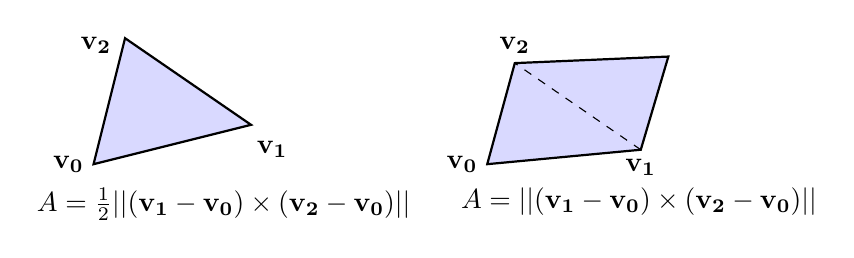
\begin{tikzpicture}[shift={(10.0,0.0)}]


  \newcommand{\mvec}[1]{\mathbf{#1}}
\newcommand{\gvec}[1]{\boldsymbol{#1}}

  \definecolor{polcol}{rgb}{0.85,0.85,1.0}

 \coordinate (v0) at (+2.0,+0.5);
 \coordinate (v1) at (+0.4,+1.6);
 \coordinate (v2) at (-0.9,+1.4);
 \coordinate (v3) at (-1.2,-0.1);
 \coordinate (v4) at (-0.5,-0.7);
 \coordinate (v5) at (+0.5,-0.8);

 \coordinate (o) at (+0.05,0.31666);

 % on the opposite side of o.
 \coordinate (r) at (2.35,1.68334);

 \tikzset{
      polstl/.style={thick,fill=polcol},
    }

% 2.35    , 1.68334
  %% triangle shift.
  \coordinate (tris) at (-5.0,0.0);

  \filldraw[polstl] (o) -- (v0) -- (r) -- (v1) -- cycle;

  \draw (o) node[left] {$\mvec{v_0}$};

  \draw (o) node[below right,xshift=-13.0,yshift=-5.0] {$A=||(\mvec{v_1}-\mvec{v_0}) \times (\mvec{v_2}-\mvec{v_0})||$};

  \draw[dashed] (v0) -- (v1);

  \draw (v0) node[below] {$\mvec{v_1}$};

  \draw (v1) node[above] {$\mvec{v_2}$};




  \filldraw[polstl] (tris) ++ (o) --  +(v0) --
  +(v1) -- cycle;

  \draw (tris) ++ (o) node[left] {$\mvec{v_0}$};
  \draw (tris) ++ (v0) node[right] {$\mvec{v_1}$};
  \draw (tris) ++ (v1) node[above left] {$\mvec{v_2}$};

  \draw (tris) ++ (o) node[below right,xshift=-24.0,yshift=-5.0] {$A=\frac{1}{2}||(\mvec{v_1}-\mvec{v_0}) \times\\ (\mvec{v_2}-\mvec{v_0})||$};


\end{tikzpicture}

\end{document}
